\chapter{Preliminaries}

This chapter will introduce the reader to the notation and definitions that will be used throughout this thesis.
This chapter is not intended to be an introduction to group theory.
It is assumed that the reader is familiar with the basics of geometric group theory, such as, presentations and Cayley graphs.
For an introduction to the basics of geometric group theory, the reader is directed to the lecture notes \cite{AMSInotes,neumann1996short} and the book \cite{clay2017office}.

\section{Basic Notation}

Within this chapter and throughout this thesis, unless otherwise stated, $G$ will denote an arbitrary group with finite generating set $X$.

\begin{definition}
	Let $x,a\in G$, then the \emph{conjugate} of $x$ by $a$, denoted $x^a$, is defined as \[ x^a = a^{-1} x a \]
\end{definition}

\begin{definition}
	Let $x,y \in G$, then \emph{commutator} of $x$ and $y$, denoted $[x,y]$, is defined as \[ [x,y] = x^{-1}y^{-1}xy \]
\end{definition}

\begin{definition}
	All group actions are \emph{left group actions}.
	For example, let $G$ act on some given set $X$, and let $g,h\in G$ and $x \in X$, then
	\[
	  ( g h ) \cdot x = g \cdot ( h \cdot x)
	\]
	That is, the right-most action, $h$, is applied first.
\end{definition}

\begin{definition}
	The \emph{free group} on a set $X$, denoted $\F(X)$, is the group generated by freely reduced words in $\left( X \cup X^{-1} \right)^\ast$, where composition is concatenation followed by free reduction.
\end{definition}

\begin{definition}
	For the purpose of this thesis the set of \emph{natural numbers}, $\mathbb{N}$, will include zero.
	\[
	  \mathbb{N}
	  =
	  \left\lbrace
	    0, 1, 2, \ldots
	  \right\rbrace
	\]
	If zero is to be excluded, then the notation $\mathbb{N}_+$ will instead be used.
\end{definition}

\begin{definition}
	A function $f : \mathbb{N} \to \mathbb{R}$ is said to be \emph{submultiplicative} if \[ f(n + m) \leq f(n) \cdot f(m) \] for each $n,m \in \mathbb{N}$.
\end{definition}

\begin{example}
	Every polynomial, $x^\alpha$ with $\alpha \geq 0$, and exponential, $\alpha^x$ with $\alpha > 1$, is submultiplicative when considered as functions that map $\mathbb{N} \to \mathbb{R}_{\geq 0}$.
\end{example}

\begin{definition}
	$\Cay(G,X)$ shall denote the \emph{Cayley graph} of $G$ with respect to a generating set $X$.
\end{definition}

\newpage
\section{Words, Lengths and Geodesics}

For any group $G$ with generating set $X$, it is possible to define a length on the elements of $G$ based on representations by words in the language $\left( X \cup X^{-1} \right)^\ast$.
This definition of length becomes important when defining the growth functions of the following section.

\begin{definition}
	\label{def:word-length}
	Let $w = w_1 w_2 \cdots w_n$ be a word where $w_1, w_2, \ldots,w_n \in \left( X \cup X^{-1} \right)$, then the \emph{word length} of $w$, denoted $\left\vert w \right\vert$, is $n$ (as $w$ is composed of exactly $n$ letters).
\end{definition}

\begin{definition}
	Let $w$ be a word in the language $\left( X \cup X^{-1} \right)^\ast$, then $\overline{w} \in G$ denotes the group element that $w$ represents.
\end{definition}

\begin{definition}
	\label{def:length}
	Let $g \in G$, then the \emph{length of $g$}, denoted $\ell_{G,X}(g)$, is defined as
	\[
	  \ell_{G,X}(g)
	  =
	  \min
	  \left\lbrace
	    \left\vert w \right\vert \in \mathbb{N}
	    \, \middle\vert \,
	    g = \overline{w}
	    \ \ 
	    \text{where}
	    \ \ 
	    w \in \left(X \cup X^{-1}\right)^\ast
	  \right\rbrace
	\]
	Under this definition, the length of the identity is defined to be zero, $ \ell_{G,X}(1_G) = 0$.
	If there is no possibility of confusion, then the $G$ and/or $X$ may be omitted from the notation.
\end{definition}

\begin{remark}
	Another way of thinking about $\ell_{G,X}(g)$ is as the distance from  $1_G$ to $g \in G$ in the Cayley graph $\Cay(G,X)$.
	\thmendmark
\end{remark}

A word is called a geodesic if it is of minimal word length for the element it represents, that is, the word length (as in \cref{def:word-length}) and the length (as in \cref{def:length}) agree.
The focus of this thesis will be generating and analysing functions which count such words.

\begin{definition}
	\label{def:geodesic}
	A word $w\in \left(X \cup X^{-1}\right)^\ast$ is called a \emph{geodesic} if $\ell_{G,X}(\overline{w}) = \left\vert w \right\vert$.
\end{definition}

\begin{remark}
	Another way of thinking of a geodesic is as a shortest path, starting at the identity, in the Cayley graph, $\Cay(G,X)$, of the group.
\end{remark}

\begin{example}
	Consider the group $C_2 \ast \mathbb{Z}$, which is the free product of the cyclic group of order two and the integers, with the presentation $\left\langle c,z \, \middle\vert \, c^2 = 1 \right\rangle$.
	Then, the word $z^2 c z^2$ is a geodesic, but $z^2 c^2 z^2$ isn't as there is a shorter word $z^4$ which represents the same group element.
\end{example}

\begin{example}
	Every freely reduced word in $\left( X \cup X^{-1} \right)^\ast$ is a geodesic in the free group $\F(X)$.
\end{example}

\begin{example}
	Consider the group $\mathbb{Z}^2$ with presentation $\left\langle x,y \, \middle\vert \, [x,y] \right\rangle$.
	Then, $x^2 y^2$ and $(xy)^2$ are length $4$ geodesics in $\mathbb{Z}^2$ which represent the same group element.
\end{example}

\begin{remark}
	From the previous example, it can be seen that geodesics are not necessarily unique, that is, there may be an element $g \in G$ with more than one corresponding geodesic.
\end{remark}

\begin{definition}
	Two words $w,v \in \left(X\cup X^{-1}\right)^\ast$ are \emph{equivalent with respect to $G$}, denoted $w =_G v$, if they represent the same group element of $G$, that is, if $\overline{w} = \overline{v}$.
\end{definition}

\begin{definition}
	Given an element $g \in G$, not necessarily a geodesic, the \emph{geodesic equivalence class} of $g$, denoted $\equivClass{g}$, is the set of all geodesics that represent $g$.
	That is,
	\[
	\equivClass{g}
	=
	\left\lbrace
	w \in \left(X \cup X^{-1}\right)^\ast
	\  \middle\vert \ 
	\overline{w} = g
	\ \ 
	\text{and}
	\ \ 
	\ell(\overline{w}) =  \left\vert w \right\vert
	\right\rbrace
	\]
	Also, given a word $w \in \left(X \cup X^{-1}\right)^\ast$, the notation $\equivClass{w}$ should be understood to mean $\equivClass{\overline{w}}$.
\end{definition}

\begin{remark}
	Given a word $w \in \left(X \cup X^{-1}\right)^\ast$, then $w \in \equivClass{w}$ if and only if $w$ is a geodesic.
\end{remark}

\begin{example}
	Consider, again, the group $\mathbb{Z}^2$ with presentation $\left\langle x,y \, \middle\vert \, [x,y] \right\rangle$.
	Then, the equivalence class $\equivClass{x^2 y^2}$ is the set of length $4$ words which contain two $x$'s and two $y$'s.
\end{example}

\newpage
\section{Growth Functions}
\label{sec:growth-functions}

The notation used in this section is a modified version of the notation used in \cite{HowGroupsGrow}.

%The definitions of each of the following growth functions should be considered with respect to some chosen group $G$ with a chosen generating set $X$.

\begin{definition}
	\label{def:strictGrowth}
	The \emph{strict growth function}, denoted $s_{G,X}$, is the function $\mathbb{N} \to \mathbb{N}$ that counts the number of elements in $G$ of length exactly $n$.
	That is,
	\[
	  s_{G,X}(n)
	  =
	  \#
	    \left\lbrace
	      g \in G
	      \ \middle\vert\ 
	      \ell_{G,X}(g) = n
	    \right\rbrace
	\]
	To simplify notation, and if there is no chance of ambiguity, the $G$ and/or $X$ may be omitted.
\end{definition}

\begin{definition}
	\label{def:cumulativeGrowth}
	The \emph{(cumulative) growth function}, denoted $\gamma_{G,X}$, is the function $\mathbb{N} \to \mathbb{N}$ that counts the number of elements in $G$ of length no more than $n$.
	That is,
	\[
		\gamma_{G,X}(n)
		=
		\#
		\left\lbrace
		g \in G
		\ \middle\vert\ 
		\ell_{G,X}(g) \leq n
		\right\rbrace
	\]
	As before, if there is no chance of ambiguity, then the $G$ and/or $X$ may be omitted.
	\thmendmark
\end{definition}

These definitions can then be modified to instead count geodesics rather than group elements.
Such functions are referred to as geodesic growth functions, and are defined as follows.

\begin{definition}
	\label{def:strictGeodGrowth}
	The \emph{strict geodesic growth function}, denoted $S_{G,X}$, is the function $\mathbb{N} \to \mathbb{N}$ that counts the number of geodesics in $G$ of length exactly $n$.
	That is,
	\[
	S_{G,X}(n)
	=
	\#
	\left\lbrace
	w \in \left(X \cup X^{-1}\right)^\ast
	\ \middle\vert\ 
	\ell_{G,X}(\overline{w}) = \left\vert w \right\vert = n
	\right\rbrace
	\]
	As before, if there is no chance of ambiguity, then the $G$ and/or $X$ may be omitted.
\end{definition}

\begin{definition}
	\label{def:cumulativeGeodGrowth}
	The \emph{(cumulative) geodesic growth function}, denoted $\Gamma_{G,X}$, is the function $\mathbb{N} \to \mathbb{N}$ that counts the number of geodesics in $G$ of length no more than $n$.
	That is,
	\[
	\Gamma_{G,X}(n)
	=
	\#
	\left\lbrace
	w \in \left(X \cup X^{-1}\right)^\ast
	\ \middle\vert\ 
	\ell_{G,X}(\overline{w}) = \left\vert w \right\vert \leq n
	\right\rbrace
	\]
	As before, if there is no chance of ambiguity,  then the $G$ and/or $X$ may be omitted.
\end{definition}

\begin{remark}
	The growth functions $\gamma_{G,X}$ and $\Gamma_{G,X}$ can be defined in terms of the strict growth functions $s_{G,X}$ and $S_{G,X}$, respectively, as follows.
	\begin{align*}
		\gamma_{G,X}(n) &= \sum_{m=0}^n s_{G,X}(m)
		&
		\Gamma_{G,X}(n) &= \sum_{m=0}^n S_{G,X}(m)
	\end{align*}
	\thmendmark
\end{remark}

In geometric group theory, the exact form of the growth function is not usually of much interest, rather, the asymptotic complexity of such functions are studied.
It is thus useful to be able to say that one growth function grows `faster' than another.
This idea is formalised as follows.

\begin{definition}
	\label{def:GrowthTotalOrd}
	Let two functions $f,g : \mathbb{N} \to \mathbb{R}_{\geq 0}$ be given.
	Then, $f$ has growth no faster than $g$, denoted $f \preccurlyeq g$, if there exists some positive constant $C \in \mathbb{N}_+$ such that \[ f(n) \leq C \cdot g\left(C \cdot n\right) \] for every $n \in \mathbb{N}_+$.
\end{definition}

\begin{remark}
	Notice the use of $\mathbb{N}_+$ rather than $\mathbb{N}$ in the previous definition.
	Although $\mathbb{N}$ would be sufficient in this case, $\mathbb{N}_+$ will be used as it is convenient for later notation.
	\thmendmark
\end{remark}

From this order, in \cref{def:GrowthTotalOrd}, an equivalence relation can be defined as follows.

\begin{definition}
	\label{def:GrowthEquivRel}
	Let two growth functions $f,g : \mathbb{N} \to \mathbb{R}_{\geq 0}$ be given.
	Then, $f$ is \emph{equivalent} to $g$, denoted $f \sim g$, if both $f \preccurlyeq g$ and $g \preccurlyeq f$ are satisfied.
\end{definition}

%\me{At some point you can reference the fact that the two functions are easily related by multiplying generating function by $\frac1{1-z}$ -- eg see my papers with Rechintzer. }

\begin{remark}
	\label{rmk:differentGrowthClasses}
	The equivalence relation of \cref{def:GrowthEquivRel} is strong enough to distinguish between polynomials and exponentials, that is, $n^\alpha \nsim \beta^n$ for every $\alpha \geq 0$ and $\beta > 1$.
	
	It is also strong enough to distinguish polynomials of different degrees, that is, $n^\alpha \nsim n^\beta$ for every $\alpha \neq \beta$ where $\alpha,\beta \geq 0$.
	
	However, this equivalence relation is not strong enough to distinguish exponentials of different bases, that is, $\alpha^n \sim \beta^n$ for  every $\alpha,\beta > 1$.
\end{remark}

\begin{proposition}[Milnor, 1968 \cite{Milnor1968}]
\label{prop:GrowthInvariant}
If $X$ and $Y$ are two generating sets for the group $G$, then $ \gamma_{G,X} \sim \gamma_{G,Y} $.
That is, the cumulative growth function is invariant under change of generating set.
\end{proposition}

\begin{remark}
	The equivalence relation of \cref{def:GrowthEquivRel} is such that if two groups $G$ and $H$ with generating sets $X$ and $Y$, respectively, are quasi-isometric to one another, then their corresponding cumulative growth functions, as in \cref{def:cumulativeGrowth}, are equivalent with respect to $\sim$.
	\thmendmark
\end{remark}

Unlike the cumulative growth function of \cref{def:cumulativeGrowth}, the cumulative geodesic growth function can vary in equivalence class depending on the chosen generating set.

\begin{example}[Example 5 from \cite{OnGroupsPolynomial}]
	Consider the group $G = \mathbb{Z} \times C_2$ where $C_2$ is the cyclic group of order two.
	Then, one potential presentation for $G$ is
	$
	  \left\langle
		  t,a
		  \, \middle\vert \,
		  a^2 = 1,\,
		  ta = at
	  \right\rangle
	$,
	which has the Cayley graph shown in \cref{fig:cg1}.
	
	\begin{figure}[h!]
		\centering
		
		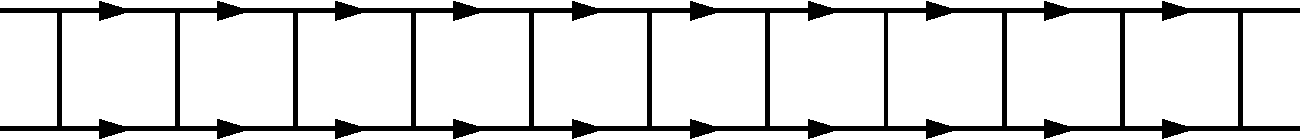
\includegraphics[width=0.85\linewidth]{figures/chapterNotation/fig1}
		
		\caption{Part of the Cayley graph for $
			\left\langle
			t,a
			\, \middle\vert \,
			a^2 = 1,\,
			ta = at
			\right\rangle
			$.}
		\label{fig:cg1}
	\end{figure}

	Performing the substitution $c = at$, the presentation
	$
	  G =
	  \left\langle
	  c,t
	  \, \middle\vert \,
	  c^2 = t^2 = 1,
	  ct = tc
	  \right\rangle
	$
	can be obtained, resulting in the Cayley graph shown in \cref{fig:cg2}.
	
	\begin{figure}[h!]
		\centering
		
		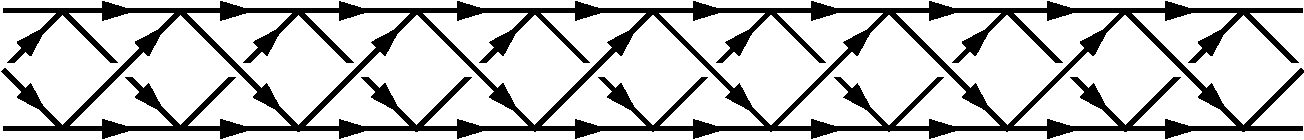
\includegraphics[width=0.85\linewidth]{figures/chapterNotation/fig2}
		
		\caption{Part of the Cayley graph for $  \left\langle
		  c,t
		  \, \middle\vert \,
		  c^2 = t^2 = 1,
		  ct = tc
		  \right\rangle$.}
		\label{fig:cg2}
	\end{figure}

	Notice that, by inspection of the two Cayley graphs, the group has polynomial geodesic growth with respect to the generating set $\left\lbrace t,a \right\rbrace$, and exponential geodesic growth with respect to the generating set $\left\lbrace c,t \right\rbrace$.
	More precisely, the group has geodesic growth $2n+2$  with respect to the generating set $\left\lbrace t,a \right\rbrace$, and geodesic growth of $2^n$  with respect to the generating set $\left\lbrace c,t \right\rbrace$.
\end{example}

\begin{example}[Example 6 from \cite{OnGroupsPolynomial}]
	A simpler example of this can be obtained by adding redundant generators to a group presentation. For example, the group formed by the integers with addition, $\mathbb{Z}$, with the usual presentation, $\left\langle z \, \middle\vert - \right\rangle$, and generating set, $\left\lbrace z \right\rbrace$, has a polynomial geodesic growth rate of $2n+1$.
	Then, by adding a redundant generator, $t$, the presentation $\left\langle z,t \middle\vert \, t = z  \right\rangle$ may be obtained, which has an exponential geodesic growth rate of $2 \cdot 2^n + 1$.
\end{example}

\begin{remark}
	Thus, by considering the previous example along with \cref{rmk:differentGrowthClasses}, it can be seen that the geodesics growth function $\gamma_{G,X}$ can vary in complexity under change of generating set.
	\thmendmark
\end{remark}

By the definition of $X$ as a generating set for $G$, it is known that for every element $g \in G$ there is at least one word $w \in \left( X \cup X^{-1} \right)^\ast$ such that $g = \overline{w}$.
Thus, the following proposition follows.

\begin{proposition}
	\label{prop:growth-function-bounds}
	The geodesic growth functions $S_{G,X}$ and $\Gamma_{G,X}$ are bounded from below by the growth functions $s_{G,X}$ and $\gamma_{G,X}$, respectively.
	Thus, both $s_{G,X} \preccurlyeq S_{G,X}$ and $\gamma_{G,X} \preccurlyeq \Gamma_{G,X}$.
\end{proposition}

\section{Intermediate Growth}
\label{sec:interGrowth}

The following definitions have been adapted from \cite{GrigPak} and \cite{HowGroupsGrow}.

Within this thesis, growth function will often be referred to as being polynomial, exponential or intermediate.
This section will define these terms with respect to the equivalence relation, $\sim$, from \cref{def:GrowthEquivRel} and the order, $\preccurlyeq$, from \cref{def:GrowthTotalOrd}.
In the following, let $f : \mathbb{N} \to \mathbb{N}$ be some arbitrary cumulative growth or cumulative geodesic growth function.

\begin{definition}
	The function $f$ is called \emph{polynomial} if there exists some $\alpha > 0$ such that $f \preccurlyeq n^\alpha$.
\end{definition}

\begin{definition}
	The function $f$ is called \emph{exponential} if $f \sim e^n$.
	\thmendmark
\end{definition}

Let $X$ be the finite generating set for the group, $G$, of which $f$ is a growth function.
Then, with $m = \left\vert X \right\vert\geq 1$, it can be seen that there can be no more than $(2m)^n$ words of length $n$ in the language $\left( X \cup X^{-1} \right)^\ast$.
Thus, there can be no more than $(2m)^n$ elements in $G$ of length $n$.
Hence,
\[
  f(n) \leq
  (2m)^0 + (2m)^1 + \cdots + (2m)^n
  \leq
  (2m)^{n+1}
\]
Thus, $f$ is always bounded from above by an exponential $(2m)^{n+1}$.

Therefore, $f$ is at most exponential in growth type, that is, $f \preccurlyeq e^n$.

Then, a growth function $f$ of \emph{intermediate growth} can be defined as one that is neither polynomial nor exponential.
To make this definition more convenient, the terms superpolynomial (a function which grows faster than any polynomial) and subexponential (a function that grows strictly slower than any exponential) will be defined; a function of intermediate growth will then be defined as one that is both superpolynomial and subexponential.

Firstly, the following lemma of cumulative growth functions will be shown.

\begin{lemma}
	The value of the limit \[ d(f) \coloneqq \limsup_{n \to \infty} \frac{\log f(n)}{\log n} \] known as the \emph{degree} of $f$, exists and lies in $\mathbb{R}_{\geq 0} \cup \left\lbrace \infty \right\rbrace$.
\end{lemma}

\begin{proof}
	Every value $\log f(n) / \log n$ of the sequence is non-negative, thus, considering that the limit superior is defined in $\mathbb{R}\cup \lbrace \pm \infty \rbrace$ for any sequence of reals, then the limit $d(f)$ exists and $d(f)\geq 0$.
	Therefore, $d(f)$ lies in $\mathbb{R}_{\geq 0} \cup \left\lbrace \infty \right\rbrace$ as required.
\end{proof}

Then, the degree $d(f)$ can be used to describe polynomial functions as follows.

\begin{proposition}
	The function $f$ is polynomial if and only if $d(f)$ is finite.
\end{proposition}

\begin{proof}
	\ \\
	$(\Longrightarrow)$
	Suppose that $f \preccurlyeq n^\alpha$, and thus there exists a constant $C \in \mathbb{N}_+$ such that $f(n) \leq C \cdot (C \cdot n)^\alpha$ for every $n \in \mathbb{N}_+$.
	Then, it follows that
	\[
	  \frac{\log f(n)}{\log n}
	  \leq
	  \frac{\log\left(C \cdot (C \cdot n)^\alpha\right)}{\log n}
	  =
	  \frac{\alpha \cdot \log n + (1+\alpha) \log C}{\log n}
	  =
	  \alpha + \frac{(1+\alpha) \log C}{\log n}
	\]
	Then, $d(f) \leq \alpha$ since $(1+\alpha)\log(C)/\log n \to 0$ as $n \to \infty$.
	Therefore, $d(f)$ is finite as required.
	
	$(\Longleftarrow)$
	Suppose that $d(f) = \beta < \infty$.
	Then, for $N \in \mathbb{N}$ sufficiently large,
	\[
	  \frac{\log f (n)}{\log n} \leq \beta + 1
	  \qquad
	  \text{for all}
	  \quad
	  n > N
	\]
	Letting $\alpha = \beta + 1$, it follows that for each $n > N$
	\[
	  \frac{\log f (n)}{\log n}
	  \leq \alpha
	  \quad
	  \Longrightarrow
	  \quad
	  \log f(n) \leq \alpha \cdot \log n
	  \quad
	  \Longrightarrow
	  \quad
	  f(n) \leq n^\alpha
	\]
	Thus, $f(n) \leq f(N) \cdot n^{\alpha}$ for all $n \in \mathbb{N}_+$.
	Therefore, $f(n) \preccurlyeq n^{\alpha}$ and is thus polynomial as required.
\end{proof}

From the previous proposition, the following definition results.

\begin{definition}
	\label{def:superpolynomial}
	The function $f$ is called \emph{superpolynomial} if $d(f) = \infty$.
	\thmendmark
\end{definition}

Now, the following lemma will be used to define subexponential growth rates.

\begin{lemma}[Grigorchuk-Pak \cite{GrigPak}]
	\label{lemma:growth-rate-bound}
	The limit
	\[
	  \omega(f) \coloneqq \lim_{n \to \infty} \frac{\log f(n)}{n}
	\]
	known as the \emph{growth rate} of $f$, always exists and has its value in $\mathbb{R}_{\geq 0}$.
	\thmendmark
\end{lemma}

The growth rate, $\omega(f)$ can then be related to the exponential growths as follows.

\begin{proposition}
	The function $f$ is exponential if and only if $\omega(f) > 0$.
\end{proposition}

\begin{proof}
	\ \\
	$(\Longrightarrow)$
	Suppose that $e^n \preccurlyeq f$, and thus there exists a constant $C \in \mathbb{N}_+$ such that $e^n \leq C \cdot f(C\cdot n)$ for all $n \in \mathbb{N}_+$.
	Then, it follows that
	\[
	  \frac{\log\left( C \cdot f(C \cdot n) \right)}{C n}
	  \geq
	  \frac{\log \left(e^n\right)}{Cn}
	  =
	  \frac{1}{C}
	\]
	Hence,
	\[
	  \frac{\log f(C \cdot n) }{Cn}
	  \geq
	  \frac{1}{C}
	  - \frac{\log C}{Cn}
	\]
	for each $n \in \mathbb{N}_+$.
	Notice that $\log C / Cn \to 0$ as $n \to \infty$.\\
	Therefore, $\omega(f) \geq 1/C > 0$ and thus $\omega(f)>0$ as required.
	
	$(\Longleftarrow)$
	Suppose that $w(f) = \beta > 0$, then for $N \in \mathbb{N}$ sufficiently large,
	\[
	  \frac{\log f(n)}{n}
	  \geq
	  \frac{\beta}{2}
	  \qquad
	  \text{for all}
	  \qquad
	  n > N
	\]
	Then, letting $\alpha = \beta/2$ it follows that $f(n) \geq e^{\alpha n} $ for all $n > N$.
	Thus, $f(n) \geq f(N) \, e^{\alpha n}$ for every $n \in \mathbb{N}_+$ and therefore $e^n \preccurlyeq f$.
	
	Then since $f \preccurlyeq e^n$, which was shown earlier in this section, it follows that $f \sim e^n$ as required.
\end{proof}

From this proposition, the following definition results.

\begin{definition}
	\label{def:subexponential}
	The function $f$ is called \emph{subexponential} if $\omega(f) = 0$.
	\thmendmark
\end{definition}

Thus, the class of intermediate growth functions can be defined as followed.

\begin{definition}
	The function $f$ is of \emph{intermediate growth} if it is both superpolynomial and subexponential as in \cref{def:superpolynomial,def:subexponential}, respectively.
\end{definition}

\begin{example}
	The function $e^{\sqrt{n}}$ is an example of intermediate growth.
	For an example of a particular group with intermediate growth, one can consider Grigorchuk's first group which was first defined by Grigorchuk in \cite{GrigFirst} and later proven to have intermediate growth in \cite{GrigInterm};
	in particular, Grigorchuk showed that this group possesses a cumulative growth $\gamma$ with
	\[
	  e^{\displaystyle \sqrt{n}}
	  \preccurlyeq
	  \gamma
	  \preccurlyeq
	  e^{\displaystyle n^{\log_{32} (31) }}
	\]
	which implies that $\gamma$ is of intermediate growth.
\end{example}


